\documentclass[11pt,answers]{exam}
\usepackage[empty]{fullpage}
\usepackage{amsmath,amssymb}
\usepackage{multicol}
\usepackage{tikz}
\usepackage{soul}

\newcommand{\ds}{\displaystyle}

\newcounter{countA}

\begin{document}
\subsubsection*{Final Exam Review - Math 243}

\begin{questions}


\question Consider the linear system below.  
\begin{align*}
\ds\frac{dx}{dt} &= x+2y \\
\ds\frac{dy}{dt} &= x 
\end{align*}

\begin{parts}

\item Re-write the system in matrix form. 
\begin{solution}
\[\dfrac{d \mathbf{x}}{dt} = \begin{bmatrix} 1 & 2 \\ 1 & 0 \end{bmatrix} \mathbf{x} \text{ where } \mathbf{x} = \begin{bmatrix} x(t) \\ y(t) \end{bmatrix}.\]
\end{solution}
\vfill

\item The eigenvectors for the system above are $\mathbf{v}_1 = \begin{bmatrix} 1 \\ -1 \end{bmatrix}$ with eigenvalue $\lambda_1 = -1$ and $\mathbf{v}_2 = \begin{bmatrix} 2 \\ 1 \end{bmatrix}$ with eigenvalue $\lambda_2 = 2$. Use these to find the general solution for the linear system. 
\begin{solution}
The general solution is 
\[
\mathbf{x}(t) = C_1 e^{-t}\begin{bmatrix} 1 \\ -1 \end{bmatrix} + C_2 e^{2t} \begin{bmatrix} 2 \\ 1 \end{bmatrix}. 
\]
\end{solution}
\vfill
\vfill

\item Find the solution to the initial value problem $x(0)  = 1$ and $y(0) = 2$.  
\begin{solution}
The solution we want has $C_1 = -1$ and $C_2 = 1$, so it is: 
\[
\mathbf{x}(t) = -e^{-t}\begin{bmatrix} 1 \\ -1 \end{bmatrix} + e^{2t} \begin{bmatrix} 2 \\ 1 \end{bmatrix}. 
\]
\end{solution}
\vfill

\end{parts}

%%%%%%%%%%%%%%%%%
%%% Problem 2 %%%
%%%%%%%%%%%%%%%%%
\question Consider the forced harmonic oscillator
$$y'' + 5y'  + 6y = 6t-1$$ 
\begin{parts}
\item Find the general solution.  
\begin{solution}
The homogeneous solution is $y_h(t) = C_1 e^{-2t} + C_2 e^{-3t}$. A particular solution is $y_p(t) = At + B$.  Then we need $5A + 6B = -1$ and $6A = 6$, so $A = 1$ and $B = -1$.  That means the general solution is
\[
y(t) = C_1 e^{-2t} + C_2 e^{-3t} + t - 1.
\]
\end{solution}
\vfill

\item If the forcing term were removed, would this oscillator be over-damped, under-damped, or critically damped?  
\begin{solution}
Overdamped (it doesn't oscillate at all). 
\end{solution}

\vfill



\end{parts}


\newpage

%%%%%%%%%%%%%%%%%
%%% Problem 3 %%%
%%%%%%%%%%%%%%%%%
\question Consider the following one-parameter family of linear systems
$$\frac{dY}{dt} = AY ~~~\mathrm{where}~~~ A = \begin{bmatrix} 2 & -a \\ 1 & 0 \end{bmatrix}.$$
\begin{parts}
\item Sketch the curve determined by the parameter $a$ in the trace-determinant plane.  
\begin{solution}
The trace is always 2, and the determinant is $a$.  So the curve is just the vertical line with $T=2$. 
\begin{center}
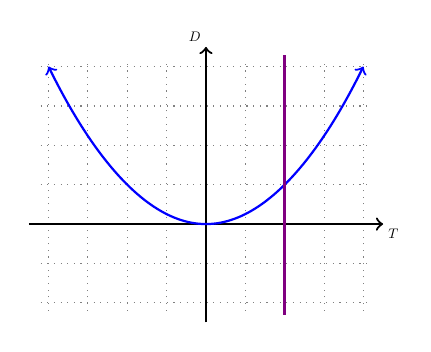
\begin{tikzpicture}[scale=0.5]
\draw[dotted,gray] (-4.2,-2.2) grid (4.2,4.2);
\draw[thick,->] (0,-2.5) -- (0,4.5) node[above left,scale=0.5] {$D$};
\draw[thick,->] (-4.5,0) -- (4.5,0) node[below right,scale=0.5] {$T$};
\draw[thick,blue,<->] (-4,4) parabola bend (0,0) (4,4);
\draw[very thick, blue!50!red] (2,-2.3) -- (2,4.3);
\end{tikzpicture}
\end{center}
\end{solution}
\vfill
\vfill

\item Describe the different types of equilibrium behaviors exhibited by the system as $a$ varies.  
\begin{solution}
When $a > 1$, we have a spiral source at the origin.  When $0 < a < 1$, we have a source, and when $a < 0$, we have a saddle. 
\end{solution}
\vfill
\end{parts}


%%%%%%%%%%%%%%%%%
%%% Problem 4 %%%
%%%%%%%%%%%%%%%%%
\question Consider the system below.  
\begin{align*}
\ds\frac{dx}{dt} &= 1 \\
\ds\frac{dy}{dt} &= 2x
\end{align*}

\begin{parts}
\item Verify that the system is a Hamiltonian system.  
\begin{solution}
If $H = y - x^2$, then $x' = H_y = 1$ and $y' = -H_x = 2x$.  
\end{solution}
\vfill

\item Find the Hamiltonian function $H$.  
\begin{solution}
The Hamiltonian function is $H = y - x^2$.
\end{solution}
\vfill

\item Use the Hamiltonian to sketch some solution curves for this system (including arrows to indicate direction).  
\begin{solution}
A level set of the Hamiltonian is a parabola $y - x^2 = C$ or equivalently $y = x^2 + C$.  The flow is always from left to right since $x' = 1$. 
\begin{center}
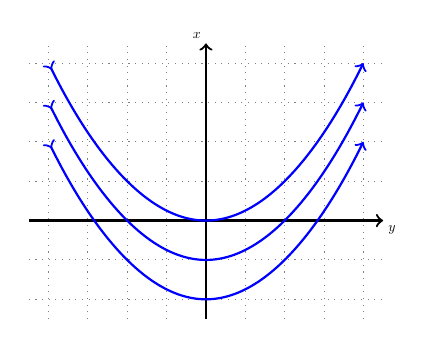
\begin{tikzpicture}[scale=0.5]
\draw[dotted,gray] (-4.5,-2.5) grid (4.5,4.5);
\draw[thick,->] (0,-2.5) -- (0,4.5) node[above left,scale=0.5] {$x$};
\draw[thick,->] (-4.5,0) -- (4.5,0) node[below right,scale=0.5] {$y$};
\draw[thick,blue,>->] (-4,4) parabola bend (0,0) (4,4);
\draw[thick,blue,>->] (-4,2) parabola bend (0,-2) (4,2);
\draw[thick,blue,>->] (-4,3) parabola bend (0,-1) (4,3);

\end{tikzpicture}
\end{center}
\end{solution}
\vfill
\vfill
\end{parts}

\newpage
%%%%%%%%%%%%%%%%%
%%% Problem 5 %%%
%%%%%%%%%%%%%%%%%
\question A patient is being treated with morphine for their pain.  The amount of morphine $y(t)$ (measured in micrograms per liter) in the patient's bloodstream after $t$ hours can be modeled by the differential equation 
$$y' + 0.1 \, y = 30 \, \delta(t - 4).$$
\begin{parts}

\item Suppose the patient initially has 100 $\mu$g/L of morphine in their blood.  In the model above, the amount of morphine in the patient would decay exponentially if it weren't for an additional injection of morphine that happens at time $t = 4$ hours.  How much extra morphine is the patient given at that time?  
\begin{solution}
The $30 \, \delta(t-4)$ terms means that 30 $\mu$g/L are being added suddenly at time $t=4$ hours.
\end{solution}
\vfill

\item Apply the Laplace transform to the differential equation above and solve for $Y(s)$.  
\begin{solution}
\[Y(s) = \dfrac{30e^{-4s} + 100}{s + 0.1}.\]
\end{solution}

\vfill

\item Solve the equation by computing the inverse Laplace transform of $Y(s)$.
\begin{solution}
\[
y(t) = 100 e^{-0.1t} + 30H(t-4) e^{-0.1(t-4)}.
\]
\end{solution}

\vfill

\end{parts}



\newpage
%%%%%%%%%%%%%%%%%
%%% Problem 6 %%%
%%%%%%%%%%%%%%%%%
\question Consider the population model
$$\frac{dP}{dt} = -\tfrac{1}{25}P^2 + 4 P - C$$
for a species of fish in a lake (here $dP/dt$ is measured in fish/year).  Here $C$ is a parameter that represents the number of fish caught per year.  
\begin{parts}
\item Draw a bifurcation diagram showing how the equilibrium fish populations depend on $C$.  Include the phase lines at three different values of $C$ (I recommend $C = 75$, 100, and something bigger than 100). 
\begin{solution}
The equilibrium points are when 
\[P = \dfrac{100 \pm \sqrt{10000 - 100 C}}{2} = 50 \pm 5 \sqrt{100 - C}.\]
These are the points on the sideways blue parabola below. 

\begin{center}
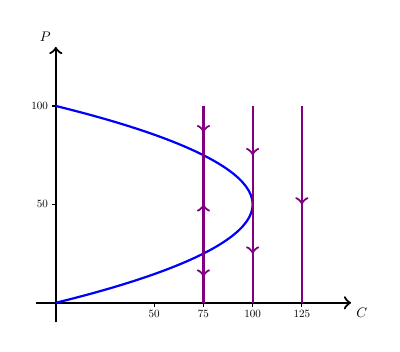
\begin{tikzpicture}[scale=0.5]
\draw[thick,->] (0,-0.5) -- (0,6.5) node[above left,scale=0.5] {$P$};
\draw[thick,->] (-0.5,0) -- (7.5,0) node[below right,scale=0.5] {$C$};
\draw (0,5) -- (-0.1,5) node[left, scale=0.4] {100};
\draw (0,2.5) -- (-0.1,2.5) node[left, scale=0.4] {50};
\draw (5,0) -- (5,-0.1) node[below, scale=0.4] {100};
\draw (2.5,0) -- (2.5,-0.1) node[below, scale=0.4] {50};
\draw (3.75,0) -- (3.75,-0.1) node[below, scale=0.4] {75};
\draw (6.25,0) -- (6.25,-0.1) node[below, scale=0.4] {125};
\draw[thick, blue, rotate=90] (0,0) parabola bend (2.5,-5) (5,0);
\draw[thick, blue!50!red] (5,0) -- (5,5);
\draw[thick, blue!50!red] (3.75,0) -- (3.75,5);
\draw[thick, blue!50!red] (6.25,0) -- (6.25,5);
\draw[thick, blue!50!red, ->] (6.25,2.8) -- (6.25,2.5);
\draw[thick, blue!50!red, ->] (5,1.5) -- (5,1.25);
\draw[thick, blue!50!red, ->] (5,3.8) -- (5,3.75);
\draw[thick, blue!50!red, ->] (3.75,4.5) -- (3.75,4.333);
\draw[thick, blue!50!red, ->] (3.75,1.0) -- (3.75,0.667);
\draw[thick, blue!50!red, ->] (3.75,2.0) -- (3.75,2.5);
\end{tikzpicture}
\end{center}

\end{solution}
\vfill
\vfill
%\begin{center}
%\includegraphics[height=3in]{final1.jpeg}
%\end{center}
\item What is the maximum catch $C$ that would still allow the fish to have a chance of survival in the lake?  
\vfill
\item Given the possibility of unexpected perturbations of the population not included in the model, what do you think would happen to the actual fish population if the yearly catch determined in part (b) was actually taken every year?  
\begin{solution}
Since the equilibrium is not stable, the population would probably collapse to zero.
\end{solution}
\vfill


\end{parts} 


\newpage
%%%%%%%%%%%%%%%%%
%%% Problem 7 %%%
%%%%%%%%%%%%%%%%%
\question A 1000 L tank is filled with salt water.  The water currently contains 20 kg of dissolved salt.  Suppose that fresh water is added to the tank at a rate of 10 L per minute and an equal amount of water drains out of the bottom so that the water level stays constant.  Assume that the water draining from the bottom is well mixed.  

\begin{parts}
\item Find a differential equation that models the amount of salt in the tank. 
\begin{solution}
Let $y(t)$ represent the kilograms of salt in the tank. The initial condition is $y(0) = 20$.  
$$\dfrac{dy}{dt} = (\text{rate in}) - (\text{rate out}) = -\tfrac{1}{100} y.$$
\end{solution}
\vfill

\item Solve the differential equation to find an equation for the amount of salt in the tank as a function of time. 
\begin{solution}
This is exponential decay, so the solution is
\[
y(t) = 20 e^{-0.01t}.
\]
\end{solution}
\vfill


\end{parts}

%%%%%%%%%%%%%%%%%
%%% Problem 8 %%%
%%%%%%%%%%%%%%%%%
\question Consider the differential equation $y' = 2 y + \cos t$.  
\begin{parts}
\item Find the general solution.  
\begin{solution}
The homogeneous solution is $y_h(t) = C e^{2t}$.  You can find a particular solution by complexifying.  Then $y_p(t)$ is the real part of 
$$\left(\dfrac{-i - 2}{5} \right) e^{it} \text{ which is } -\tfrac{2}{5} \cos t + \tfrac{1}{5} \sin t.$$ 
So the general solution is 
$$y(t) = C e^{2t} - \tfrac{2}{5} \cos t + \tfrac{1}{5} \sin t.$$
\end{solution}

\vfill
\item Solve the initial value problem $y(0) = 0$. 
\begin{solution}
$$y(t) = 2 e^{2t} - \tfrac{2}{5} \cos t + \tfrac{1}{5} \sin t.$$
\end{solution}

\vfill
 

\end{parts}
\newpage

%%%%%%%%%%%%%%%%%
%%% Problem 9 %%%
%%%%%%%%%%%%%%%%%
\question Consider the differential equation $\ds \frac{dy}{dt} = 3y^{2/3}$.  
\begin{parts}
\item Verify that $y(t) = 0$ is a solution to the differential equation.  
\begin{solution}
The derivative of zero is zero and $3(0)^{2/3} = 0$.  So both sides are equal.
\end{solution}
\vfill

\item Verify that $y(t) = t^3$ is also a solution to the differential equation.
\begin{solution}
$\dfrac{d}{dt} t^3 = 3 t^2$ which is the same as $3(t^3)^{2/3}$.  So both sides are equal.
\end{solution}
\vfill

\item One of the most important theorems about differential equations is the following: \\

\textbf{Uniqueness Theorem}. \emph{If $\dfrac{dy}{dt} = f(t,y)$ is a differential equation where both $f$ and its partial derivative $f_y$ are continuous for all points $(t,y)$ near $(t_0,y_0)$, then there exists a unique solution $y(t)$ defined on an open interval around $t_0$ such that $y(t_0) = y_0$.  } \\

Given that solutions of a differential equation are supposed to be unique, how is it possible that the differential equation above has two different solutions that pass through the point $(0,0)$?  Explain why this does not contradict the Uniqueness Theorem. 
\begin{solution}
The Uniqueness Theorem doesn't apply here since the partial derivative $\dfrac{\partial}{\partial y} 3y^{2/3} = \dfrac{2}{y^{1/3}}$ which is not continuous at $y = 0$.  
\end{solution}

\vfill

\end{parts}

\newpage
%%%%%%%%%%%%%%%%%%
%%% Problem 10 %%%
%%%%%%%%%%%%%%%%%%
\question Consider the following nonlinear system of equations.
\begin{align*}
\ds\frac{dx}{dt} &=  x^2-y \\
\ds\frac{dy}{dt} &=  2y^2-2 
\end{align*}

\begin{parts}

\item Identify all of the equilibrium points for this system. 
\begin{solution}
The equilibria are $(-1,1)$ and $(1,1)$.  
\end{solution}
\vfill

\item Find the Jacobian matrix at each equilibrium and use it to classify the type for each (sink, source, spiral sink, spiral source, or saddle).  
\begin{solution}
The Jacobian is $\begin{bmatrix} 2x & -1 \\ 0 & 4y \end{bmatrix}$.  At $(-1,1)$ is has a positive and a negative eigenvalue, so that is a saddle.  At $(1,1)$, both eigenvalues are positive, so it is a source. 
\end{solution}

\vfill

\vfill
\end{parts}
%%%%%%%%%%%%%%%%%%
%%% Problem 11 %%%
%%%%%%%%%%%%%%%%%%
\question  Consider the linear system
$$\frac{dY}{dt} = \begin{bmatrix} -4 & 3 \\ -3 & -4 \end{bmatrix}\, Y.$$
\begin{parts}
\part Verify that $\begin{bmatrix} 1 \\ i \end{bmatrix}$ as an eigenvector of $\begin{bmatrix} -4 & 3 \\ -3 & -4 \end{bmatrix}$.  What is its corresponding eigenvalue? 
\begin{solution}
\[
\begin{bmatrix} -4 & 3 \\ -3 & -4 \end{bmatrix} \begin{bmatrix} 1 \\ i \end{bmatrix} = \begin{bmatrix} -4 + 3i \\ -3 -4i \end{bmatrix} = (-4 + 3i) \begin{bmatrix} 1 \\ i \end{bmatrix}.
\]
The corresponding eigenvalue is $-4 + 3i$. 
\end{solution}
\vfill

\part Find the general (real-valued) solution of the system above.
\begin{solution}
The real and imaginary parts of $e^{(-4 + 3i)t} \begin{bmatrix} 1 \\ i \end{bmatrix}$ are both solutions. So the general solution is
\[
Y(t) = C_1 e^{-4t} \begin{bmatrix} \cos 3t \\ - \sin 3t \end{bmatrix} + C_2 e^{-4t} \begin{bmatrix} \sin 3t \\ \cos 3t \end{bmatrix}.
\]
\end{solution}
\vfill
\end{parts}

\newpage


\end{questions}

\end{document}
